\newpage
\subsection{Vis new rule}
\visHeader

\begin{figure}[htp]
\begin{center}
  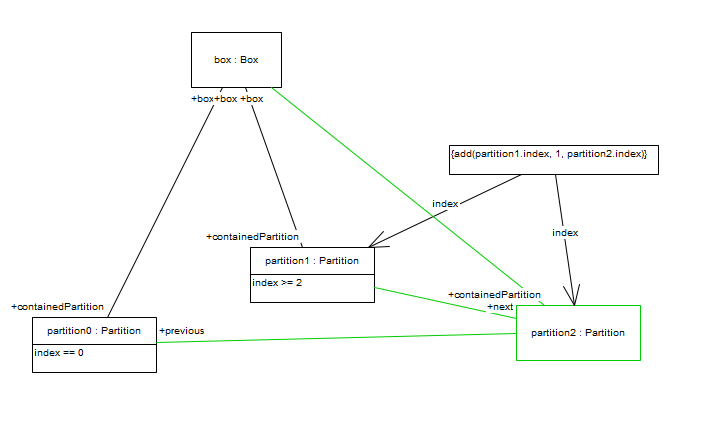
\includegraphics[width=\textwidth]{allOtherCardsRule}
  \caption{figureCaption \update change to n, n+1}
  \label{fig:allOtherCardsRule}
\end{center}
\end{figure}

When the \texttt{BoxToDictionary} doesn't work, this comes into play. It find the starter position then matches to a partition, n. You can see from the
constraint that the index for the additional partition adds 1 to n, so that the newest partition becomes n+1. Remember, the black are things that are already
established. The green indicates that there is no object like that currently in the transformation.